\documentclass[twocolumn,10pt]{article}

% ---------- layout to mirror an ACM-workshop-style two-column paper ----------
\usepackage[letterpaper,top=0.9in,bottom=1in,left=0.75in,right=0.75in,columnsep=0.28in]{geometry}
\usepackage[T1]{fontenc}
\usepackage{amsmath}
\usepackage{mathptmx}
\usepackage{microtype}
\usepackage{graphicx}
\usepackage{booktabs}
\usepackage{array}
\usepackage{tikz}
\usetikzlibrary{positioning,arrows.meta,calc}
\usepackage[superscript,nospace,nocompress]{cite}
\usepackage{caption}
\captionsetup{font=small,labelfont=bf,labelsep=period}
\usepackage{titlesec}
\titleformat{\section}{\large\bfseries}{\thesection}{0.8em}{}
\titleformat{\subsection}{\normalsize\bfseries}{\thesubsection}{0.7em}{}
\titlespacing{\section}{0pt}{*2.2}{*1.1}
\titlespacing{\subsection}{0pt}{*1.8}{*0.9}
\usepackage[hidelinks]{hyperref}
\hypersetup{pdftitle={Using Predictable Orbits to Synchronize Clocks in Orbital Data Centers},pdfauthor={Ming Leong Tsui}}
\urlstyle{same}
\usepackage{etoolbox}
\makeatletter
\renewcommand\@biblabel[1]{#1.}
\makeatother
\setlength{\parskip}{0pt}
\frenchspacing

% run-in paragraph headings like the model paper's research-opportunities section
\newcommand{\runin}[1]{\smallskip\noindent\textit{#1.}\hspace{0.6em}}

\title{\LARGE\bfseries Using Predictable Orbits to Synchronize Clocks in Orbital Data Centers}
\author{%
Ming Leong Tsui\\
\normalsize Boston University\\
\normalsize Boston, MA, USA}
\date{\normalsize June 2026}

\begin{document}

\maketitle

% ====================================================================
\begin{abstract}
\noindent
A data center built from thousands of satellites requires its machines to agree on the time, because distributed software relies on synchronized clocks to order events, keep replicated data consistent, and share schedules. The time architecture satellites inherit today, that of the Global Positioning System, keeps time on the ground, depending on a set of atomic clocks under nearly continuous ground supervision and broadcasting time one way to passive receivers. An orbital data center requires a different design, since it flies thousands of commodity clocks that a ground station sees for only minutes per day, and its software needs the satellites to agree with one another rather than with an outside authority. Although installing a GNSS receiver on every satellite is a proven solution to the problem, the received time then depends on a signal outside the operator's control, one that can be jammed, spoofed, or denied. We propose that this dependence is unnecessary if the constellation keeps time by itself over the inter-satellite laser links it already operates. Orbital motion is predictable, so the dominant error in a clock comparison between two satellites, namely their own motion during the exchange, can be computed from the orbit predictions every operator already maintains and subtracted from the measurement, reducing it from hundreds of nanoseconds to below a picosecond, beneath the timestamping floor of the link hardware. The synchronization schedule itself can likewise be computed a full orbital period in advance rather than discovered at runtime. The fleet can therefore hold nanosecond mutual agreement on commodity clocks with no external signal. That time is served to onboard software as an interval carrying an explicit uncertainty bound, which lets the software order events and share link schedules safely, with a bound that widens gracefully when a satellite is cut off instead of failing silently. We state the conditions under which other time-synchronization designs become preferable and lay out a falsifiable evaluation agenda.
\end{abstract}

\section{Introduction}\label{sec:intro}
Computation is moving into low Earth orbit. As of June 2026 SpaceX operates more than ten thousand working Starlink satellites~\cite{mcdowellstats}, joined by inter-satellite links, or ISLs, through a mesh of roughly nine thousand laser terminals that carried beyond forty petabytes per day at one hundred gigabits per link in early 2024~\cite{brashears2024}. Denby and Lucia argued in 2020 that a constellation should be treated as a computer system rather than a fleet of bent-pipe relays, because downlink capacity cannot keep up with sensor data and processing must happen in orbit~\cite{denby2020}. The thought experiment of putting server-grade compute in orbit was taken seriously the same year~\cite{bhattacherjee2020}, and by late 2025 it had left the realm of thought experiments entirely. Google announced Project Suncatcher, a planned constellation of solar-powered satellites carrying machine-learning accelerators linked by free-space optics~\cite{suncatcher2025}, Starcloud flew a data-center-class GPU~\cite{starcloud2025}, and in January 2026 SpaceX filed with the FCC for an orbital data center constellation of up to one million satellites~\cite{spacenews2026}. The orbital data center has stopped being a metaphor.

A computer made of thousands of moving nodes faces operating-system problems, and synchronization carries the others. Processes on different satellites that exchange messages, share state, schedule a link, or hand off a role need to order events, and ordering needs either communication or time~\cite{lamport1978,liskov1991}. Communication in a constellation is the expensive, churning resource. Links break and reform as planes rotate past each other, paths stretch and shrink by milliseconds~\cite{kassing2020}, and radiation-induced faults arrive as unscheduled reboots~\cite{pfandzelter2023}. Synchronized clocks are the one coordination mechanism whose cost does not grow with topology churn, because a clock keeps working while a link is down. This is why we treat synchronization as the part of inter-process communication to solve first.

GPS is a magnificent answer to a different question, and the instinct to inherit its time does not transplant into this regime. It distributes absolute time from a few dozen premium clocks, corrected by a ground segment that sees every satellite nearly continuously, to passive receivers that never talk back~\cite{ashby2003,gpscontrol}. An orbital data center inverts every term of that sentence. We make the inherited assumptions explicit in Section~\ref{sec:gps} and show in Section~\ref{sec:breaks} that scale, hardware class, geometry, relativity, and the identity of the time consumer all move against them.

We concede the obvious shortcut before building anything. Every satellite can carry a GNSS receiver and inherit absolute time at the tens-of-nanoseconds level~\cite{pod,fccgen2}, and we derive in Section~\ref{sec:buys} that ordering correctness between satellites needs agreement only at the light time separating them, which bottoms out near seventy microseconds at the closest approach of a dispersed shell and at a third of a microsecond in close formation, bars GNSS clears by orders of magnitude. An operator willing to rest a fleet's ordering on an external signal can keep a receiver per satellite plus a holdover oscillator and stop there. What remains after that concession defines the contribution. The diagnostic layer still applies, because GNSS hands a satellite a time value while the relativistic rates, maneuver steps, and thermal drifts of Section~\ref{sec:breaks} keep corrupting how the satellite carries that value between fixes. The interval discipline stands on its own, because a bound that widens under degradation is safer than a value that drifts unflagged. Only the exchange fabric is specific to the operator unwilling to accept the dependence, the posture that led BeiDou to fly its own crosslink time comparison instead of borrowing GPS~\cite{li2025}.

For that operator, orbital predictability offsets what scale takes away. The dominant error in a two-way time exchange between two satellites is their motion during the exchange, which biases the measurement by up to hundreds of nanoseconds. That motion follows orbital mechanics, and navigation practice has corrected two-way time transfer with predicted orbits for decades~\cite{itu1153,li2025}. We show in Section~\ref{sec:method} what the correction yields in the commodity regime, a residual below a picosecond at the velocity knowledge onboard navigation already delivers, three orders of magnitude under the hardware timestamping floor. Satellites sharing a circular shell tick at the same relativistic rate to first order, so a constellation-wide timescale is even well defined, something no terrestrial data center gets for free. The same determinism lets the synchronization schedule be computed ahead for a full orbital period instead of discovered at runtime.

We propose constellation time, an architecture with three commitments. Time is served as an interval with an explicit uncertainty bound in the style of Spanner's TrueTime~\cite{corbett2012}. The bound is maintained by scheduled two-way exchanges over the constellation's existing ISLs, fused with GNSS and gateway anchors when they are available and explicit about uncertainty when they are not. And geometry enters the protocol as a correction input, computed from ephemerides. Section~\ref{sec:risks} bounds the GNSS objection quantitatively, names the further ways this could be wrong, and states the evidence that would make us abandon the fabric and keep only the layers above it. Section~\ref{sec:related} positions the proposal against navigation-system practice and data-center synchronization. Every computed value in this paper is reproduced by a single derivation script.\footnote{The script accompanies this paper and recomputes all orbital geometry, relativistic rates, and error budgets from physical constants.}

\section{Background}\label{sec:background}
\subsection{From Relays to Orbital Data Centers}\label{sec:relays}
The case for computing in orbit is older than the current commercial wave. Denby and Lucia showed that a bent-pipe architecture, in which satellites merely sense and downlink, saturates ground-link capacity and leaves most collected data undeliverable, and they proposed orbital edge computing on commodity hardware as the alternative~\cite{denby2020}. Their computational nanosatellite pipelines are an early and instructive use of orbital determinism, because the pipeline parallelism they propose only works because satellites in a shared orbit hold formation predictably. Bhattacherjee and colleagues asked whether full server-grade computation in orbit is outlandish and concluded that power, thermal management, and launch cost present challenges, none prohibitive~\cite{bhattacherjee2020}.

The 2025 generation of orbital compute targets data-center workloads outright. Google's Project Suncatcher proposes constellations of solar-powered satellites carrying tensor processing units, flown in close formation and meshed with free-space optical links, explicitly framed as a path to scaling machine-learning infrastructure~\cite{suncatcher2025}. Starcloud flew an H100-class GPU in late 2025 and markets orbital data centers as its product~\cite{starcloud2025}. SpaceX's January 2026 filing proposes up to one million satellites between 500 and 2{,}000 km for the same purpose, with the company asserting that the lowest cost to generate AI compute will soon be in space~\cite{spacenews2026}. The economics need sober treatment, and a 2026 JPL analysis finds that launch costs remain a factor of three to fourteen too high for orbit to substitute for terrestrial data centers, while judging space-native processing and communications-integrated compute to be credible early regimes~\cite{turyshev2026}. Those early regimes are the ones this paper assumes, computation that lives on constellation hardware because its data or its network lives there first.

Published orbital-compute designs do not treat synchronization. Google's Suncatcher design analyzes optical link budgets, formation-flying dynamics, radiation tolerance of accelerators, and launch economics in detail, and we find no treatment of clock synchronization or distributed time in it~\cite{suncatcher2025}. Denby and Lucia's pipelines handle time carefully but only as per-satellite bookkeeping, using predictability to eliminate inter-satellite coordination rather than to support it~\cite{denby2020}, a design point that works for independent sensing pipelines and stops working the moment satellites share mutable state over ISLs. The omission makes sense, since nothing in a constellation works without power, links, and radiation tolerance. The gap still matters, because nothing distributed works correctly without ordering.

A constellation that computes is simultaneously the computer and the network, and that dual role makes its operating-system problems unusual. The inter-satellite topology amounts to a physical schedule. Optical terminals take seconds to acquire, which is why deployed and studied constellations fly static grid topologies~\cite{pfandzelter2023,bhattacherjee2019}. Link capacity, beam pointing, and medium access are therefore scheduled resources, and schedules presuppose a shared clock. Synchronization in an orbital data center consequently gates the network that everything else, including synchronization itself, runs over. Predictability dissolves the circularity, because the schedule that needs time can be computed without it, from geometry alone.

\subsection{What Synchronized Clocks Are For}\label{sec:clocksfor}
Ordering events is the base primitive of inter-process communication, and physical time is one of two ways to get it. Lamport's happened-before relation orders events through message causality alone, and the same paper names the failure mode, anomalous behavior, in which causality flows through channels outside the system where logical clocks cannot see it~\cite{lamport1978}. An orbital data center is full of outside channels, ground operators, user terminals, sensed phenomena, other constellations, so physical time becomes a hard requirement. Synchronized clocks then remove messages outright, the classic catalog being leases, at-most-once delivery, and cache consistency~\cite{liskov1991}, and message removal is worth most where messaging is fragile, in a system whose links break and reform on schedule.

Terrestrial data centers treat clock uncertainty as a first-class quantity, and we extend that lineage. TrueTime serves intervals guaranteed to contain true time and waits them out for external consistency~\cite{corbett2012}, Huygens reaches tens of nanoseconds on commodity network-interface timestamps~\cite{geng2018}, Sundial holds a roughly hundred-nanosecond worst-case bound under failures and argues that the bound is the deliverable~\cite{li2020}, and hybrid logical clocks mark what remains achievable with no trustworthy bound at all~\cite{kulkarni2014}. The deliverable we carry into orbit is the same, a bound that is small, available, and never silently wrong.

\section{How GPS Keeps Time}\label{sec:gps}
GPS time is manufactured on the ground. A master control station and a network of seventeen globally distributed monitoring sites track every satellite, estimate each satellite clock's offset and drift against a ground ensemble, and upload correction coefficients that the satellite then broadcasts to users~\cite{gpscontrol}. The architecture asks the satellite for predictability rather than correctness, and the ground segment converts that predictability into corrections. GPS time itself is a paper timescale steered toward UTC as maintained by the United States Naval Observatory, with a published commitment of thirty nanoseconds at the ninety-fifth percentile~\cite{gpssps}.

Premium onboard clocks are what make the sparse correction loop viable. Each GPS satellite carries multiple cesium or rubidium atomic frequency standards whose fractional stability allows an upload cadence of once per day to hold user-range error within specification~\cite{gpssps,ashby2003}. The architecture spends mass, power, and money on the clock so that it can spend almost nothing on the control loop. This trade is available because the constellation is small, and a few dozen flight-qualified atomic standards are an affordable line item.

Relativity is engineered in once, at design time. A clock in the GPS orbit gains about 45.7 microseconds per day from the weaker gravitational potential and loses about 7.1 microseconds per day from time dilation, and left uncorrected the net offset would walk positioning off by more than eleven kilometers per day~\cite{pascual2005}. The remedy is a single factory adjustment. The clock frequency is offset by the net fractional rate of $4.4647\times10^{-10}$ before launch, to 10.229\,999\,995\,43 MHz against a nominal 10.23 MHz, so that the broadcast arrives on rate at the geoid~\cite{ashby2003}. Orbital eccentricity adds a periodic term that the receiver removes with a standard correction, about 23 nanoseconds in amplitude at an eccentricity of 0.01, and Earth rotation enters as the Sagnac correction, hundreds of nanoseconds depending on geometry~\cite{ashby2003}.

Time then flows in one direction only. A receiver treats its own clock error as a fourth unknown solved alongside three coordinates, which is why GPS satellites never need to agree with each other directly and never accept time from below~\cite{ashby2003,pascual2005}.

This architecture encodes assumptions worth naming, because each one fails in orbit-as-data-center. We make them explicit. First, clocks are premium payloads, few in number. Second, a ground segment sees every satellite essentially continuously and owns the correction loop. Third, time flows one way to passive external users, so satellites need no mutual agreement. Fourth, the relativistic environment is a design constant, set once for a single orbit class. Fifth, the consumer of time is outside the system and wants absolute traceable time, while the satellites themselves need no mutual agreement. Table~\ref{tab:assumptions} summarizes the set against the orbital data center reality established next.

\begin{table}[t]
\centering
\small
\begin{tabular}{@{}p{1.55cm}p{2.85cm}p{2.9cm}@{}}
\toprule
 & \textbf{GPS} & \textbf{Orbital data center} \\
\midrule
clocks & atomic standards as payload & commodity oscillators as bus parts \\
control & ground sees every satellite continuously & one station sees a satellite 0.5\,\% of the time \\
time flow & one-way broadcast to passive receivers & mutual agreement across ISLs \\
relativity & one constant offset set at the factory & modeled continuously from ephemerides \\
consumer & external, wants absolute time & internal, wants bounded mutual time \\
\bottomrule
\end{tabular}
\caption{Architectural assumptions of GPS timekeeping and their replacements in an orbital data center.}
\label{tab:assumptions}
\end{table}

\section{What No Longer Holds in an Orbital Data Center}\label{sec:breaks}
Each GPS assumption fails separately, and for a different physical reason, when the constellation becomes the computer. This section walks through the failures in the order of Table~\ref{tab:assumptions} and quantifies each one. The section reads the inherited architecture on its own terms, a constellation keeping time without leaning on external signals, and Section~\ref{sec:risks} prices the per-satellite-receiver alternative that a GNSS-trusting operator would choose instead. The arithmetic uses a representative shell modeled on the deployed Starlink first shell, with 1{,}584 satellites in 72 planes of 22 at 550 km altitude and 53 degrees inclination~\cite{kassing2020}, an orbital radius of 6{,}921 km, an orbital speed of 7.59 km/s, and a period of 95.5 minutes.

\subsection{The Ground Segment Loses Its View}\label{sec:break-control}
Ground-centric correction assumes the ground can watch every clock almost continuously, and at 550 km it cannot. A GPS satellite at 26{,}562 km radius is above the horizon for a single ground station across 76 degrees of Earth-central angle, which covers 38 percent of the planet's surface, so a modest global network of monitor stations keeps every satellite in essentially continuous view~\cite{gpscontrol}. A satellite at 550 km with a 25-degree elevation mask is visible within an Earth-central angle of 8.5 degrees, which covers 0.54 percent of the surface. The masks differ deliberately, since gateway links need elevation while the GPS figure describes horizon visibility, and the contrast holds under any like-for-like choice, 38 against 4.0 percent at the horizon and 19.5 against 0.54 percent at 25 degrees. A pass over one station tops out near five minutes of a 95.5-minute orbit, Earth rotation included. Per satellite and per station, contact is rare and brief.

Scale then multiplies the orphaned-clock problem by four orders of magnitude. The architecture that hand-corrects a few dozen premium clocks does not extend to many thousands of commodity ones, and the fleet sizes have arrived, with more than ten thousand working Starlink satellites~\cite{mcdowellstats}, a second constellation of 3{,}232 planned satellites deploying since April 2025~\cite{kuiper}, and the ground-station bottleneck named in the ISL literature as the constraint that even telemetry collection runs into~\cite{wu2024}. The ground keeps its anchor role, because gateways still tie the fleet to UTC and at fleet level some satellite essentially always sits over some gateway. The correction loop inverts all the same. A constellation that declines external time must keep itself synchronized between anchor contacts and carry anchor time across the grid, a function GPS never asked of its space segment, while a constellation content with GNSS outsources both the function and the dependence to receivers.

\subsection{The Clock Becomes a Commodity Part}\label{sec:break-clock}
An orbital data center will not fly an atomic frequency standard per node, because its economics are built on commodity hardware~\cite{denby2020,bhattacherjee2020}. The oscillators that actually fly on LEO missions are temperature-compensated and oven-controlled crystals, with the best oven-controlled units reaching short-term stability near $10^{-12}$ and the ultra-stable oscillators of science missions reaching one to three parts in $10^{13}$ between ten and a thousand seconds~\cite{wang2022}. Chip-scale atomic clocks add an atomic reference at about 120 mW of power, with stability of $10^{-11}$ at a thousand seconds and aging under $9\times10^{-10}$ per month~\cite{csac}, cheap enough to fly on every node but still orders of magnitude away from the navigation-grade standards the GPS correction cadence was designed around. Free-running time uncertainty grows as the frequency error times the elapsed time, so a $10^{-7}$ oscillator accumulates a microsecond of uncertainty in ten seconds, while a calibrated $10^{-11}$ clock needs seventeen minutes to drift ten nanoseconds. Oscillator class therefore sets the refresh cadence a synchronization service must sustain, and it sets what remains when a satellite is cut off. Under continuous GNSS discipline this arithmetic prices outages only, and without external time it prices everything.

The orbital environment also attacks the clock subsystem directly, in two periodic and one stochastic way. A satellite at 550 km enters Earth's shadow for up to 35.6 minutes of every 95.5-minute orbit, so the thermal environment of the oscillator cycles with the orbital period, and oscillator frequency follows temperature. Radiation adds the stochastic part. Estimated single-event-upset rates for constellation-scale COTS compute imply tens to hundreds of upset-induced faults per day across a Starlink-sized fleet, and from the software's perspective these arrive as unscheduled reboots~\cite{pfandzelter2023}. A reboot destroys clock discipline state, so the synchronization architecture must treat a satellite that suddenly knows nothing about time as routine.

\subsection{The Consumer of Time Moves Into Orbit}\label{sec:break-consumer}
GPS serves absolute time outward to passive receivers, but an orbital data center consumes time inward, between its own processes. Replicated state, distributed transactions, lease-based ownership, telemetry correlation, and the medium-access schedule of the ISLs themselves all need satellites to agree with each other within a known bound~\cite{corbett2012,liskov1991}. Mutual agreement is a different deliverable than absolute accuracy. A pair of satellites that are both wrong about UTC by the same amount can still order events, hold leases, and share a TDMA frame perfectly well, while a pair that is individually accurate on average but occasionally unbounded cannot safely do any of those things~\cite{li2020}.

Message-based synchronization inherits the network's geometry, and in orbit that geometry moves. Round-trip times between fixed endpoints through a LEO shell change by factors approaching two within minutes, with discrete jumps when paths reroute~\cite{kassing2020}, and inter-satellite latencies sit at milliseconds against the microseconds of a terrestrial fabric~\cite{bhattacherjee2020}. An NTP-style exchange that assumes symmetric, stable paths~\cite{mills1991} faces a medium whose asymmetry is real, large, and changing. The saving grace is that the change is deterministic.

\subsection{The Geometry Will Not Hold Still}\label{sec:break-geometry}
Inter-satellite link geometry in a shell is dynamic in a structured way, and the structure is worth stating exactly, because it sets the error budget of any time transfer that runs over the links. Within one orbital plane, satellites rotate rigidly, so the range between intra-plane neighbors, 1{,}970 km in the representative shell, is constant to numerical roundoff. Between adjacent planes the range oscillates each orbit, and the range rate between cross-plane grid neighbors peaks between roughly 90 and 260 m/s depending on the phasing offset between planes. Links between satellites on crossing tracks are qualitatively different. Two satellites of a 53-degree shell on ascending and descending passes close on each other at up to $2v\sin i$, which is 12.1 km/s, and this is one reason deployed topologies connect only gentle neighbors in a static grid~\cite{bhattacherjee2019,pfandzelter2023}. Figure~\ref{fig:isl} shows one orbit of cross-plane neighbor geometry.

Motion during a time-transfer exchange biases the measurement. A two-way exchange estimates the clock offset between two satellites by assuming the path is the same length in both directions. When the range changes at rate $\dot\rho$ during an exchange whose one-way flight time is $d$ and whose turnaround is $\tau$, the two directions see different path lengths, and the estimate acquires a bias of $\dot\rho\,(d+\tau)/2c$. We quote a deliberately padded envelope case, 350 m/s on a 1{,}300 km link with a 5 ms turnaround, for a bias of 5.4 ns, while the worst actual grid link in the representative shell stays under 3 ns. On a crossing link at 12 km/s the bias reaches 234 ns. Uncorrected, satellite motion dominates orbital time transfer by one to three orders of magnitude over the hardware floor. The term follows directly from the ephemeris, and navigation practice corrects it as routine~\cite{itu1153,li2025}.

\begin{figure}[t]
\centering
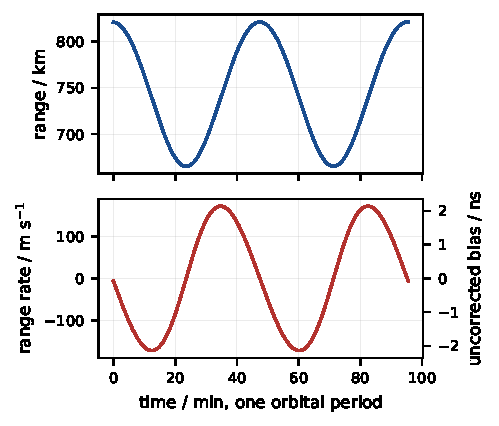
\includegraphics[width=\columnwidth]{figs/fig_isl.pdf}
\caption{One orbital period of geometry between adjacent-plane grid neighbors in a 72-plane, 22-satellite shell at 550 km and 53 degrees with phasing offset 11. Range oscillates by roughly 160 km and the range rate stays within about 170 m/s, gentle by orbital standards yet worth single nanoseconds of two-way bias if ignored, with crossing links worth hundreds. The right axis of the lower panel converts range rate to uncorrected two-way bias for a 5 ms turnaround at this link's mean range.}
\label{fig:isl}
\end{figure}

\subsection{Relativity Changes Sign and Becomes Operational}\label{sec:break-relativity}
The relativistic clock-rate offset at LEO altitude is opposite in sign to the GPS case and similar in size, so it cannot be ignored and cannot be inherited. For a circular orbit the fractional rate against a geoid clock is $y(r)=\bigl(W_0-\tfrac{3GM}{2r}\bigr)/c^2$, where the single combination $\tfrac{3}{2}GM/r$ captures both the gravitational potential and the orbital velocity, because $v^2=GM/r$. Evaluating it reproduces the GPS value of $+38.6$ microseconds per day, places the null shift at 3{,}175 km of altitude, and gives $-22.8$ microseconds per day at 550 km. A LEO clock runs slow where a GPS clock runs fast, because below the null altitude the velocity term wins. Figure~\ref{fig:rates} plots the whole curve, and both of its anchors check against Ashby, who publishes the same GPS rate and a null-shift radius near 9{,}545 km~\cite{ashby2003}.

\begin{figure}[t]
\centering
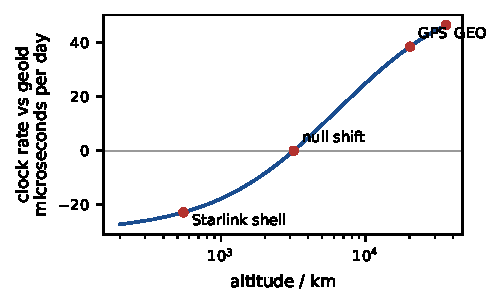
\includegraphics[width=\columnwidth]{figs/fig_rates.pdf}
\caption{Fractional clock rate against a geoid clock for circular orbits, evaluated from $y(r)=(W_0-\tfrac{3}{2}GM/r)/c^2$. The curve crosses zero near 3{,}175 km altitude. GPS clocks run fast by 38.6 microseconds per day while clocks in a 550 km shell run slow by 22.8, an offset of the same order with the opposite sign.}
\label{fig:rates}
\end{figure}

Relativity also stops being a single factory constant and becomes a continuously modeled, per-satellite quantity. The burden is that the rate offset depends on the orbit actually flown, with a sensitivity of 12 nanoseconds per day per kilometer of altitude at 550 km, so shells thirty kilometers apart drift hundreds of nanoseconds per day relative to each other, drag decays altitude continuously, and collision-avoidance maneuvers shift altitude by one to three kilometers at a time~\cite{pfandzelter2023} and therefore step the clock rate by tens of nanoseconds per day. The maneuver tempo is also rising fast, from an average of twelve per satellite per year in 2022~\cite{pfandzelter2023} to a fleet total of 144{,}404 in the six months ending May 2025~\cite{maneuvers2025}, which works out to roughly thirty per satellite per year. Periodic terms exist too, though they are small. Eccentricity below $10^{-3}$ keeps the periodic eccentricity term under 1.2 ns of amplitude, and the Earth-oblateness term stays below half a nanosecond at twice the orbital frequency. All of it is computable from the ephemerides the operator already maintains. The gift is that satellites sharing one circular shell share one value of $r$, so to first order they share one proper-time rate, and a single constellation-wide timescale is physically well defined across the shell. The first-order label carries weight, because satellites a kilometer apart in altitude still drift apart by 12 nanoseconds per day, a modeled term like the rest. GPS exploits the shared rate only once, as the common factory offset, and never defines its operational timescale on it, since the ground corrects each clock individually anyway. In an orbital data center the common rate means that once clocks are aligned, hardware drift rather than physics pulls them apart, and a synchronization fabric can measure and remove exactly that drift.

\section{Constellation Time}\label{sec:method}
We propose constellation time, a synchronization architecture for orbital data centers built on three commitments. First, the service hands software time as an interval with an explicit uncertainty bound rather than as a bare number. Second, the bound is maintained by two-way exchanges over the inter-satellite links the constellation already flies, with all geometric and relativistic corrections computed from ephemerides. Third, the exchange schedule, the anchor schedule, and the failure-recovery structure are computed ahead of time for a full orbital period, because in this system the future topology comes from ephemerides the operator already publishes. Figure~\ref{fig:arch} shows the resulting stack. The architecture maintains two timescales, an internal constellation timescale that satellites agree on tightly, and a steering relationship to UTC through anchors, mirroring how GPS time itself is a paper timescale steered toward UTC rather than identical to it~\cite{gpssps}. The layers separate cleanly. The interval contract and the dynamics model serve any time source, plain GNSS included, while the exchange fabric adds the one path free of outside reference. Section~\ref{sec:ipc} then sketches the communication and state layer the whole service exists to support.

\begin{figure}[t]
\centering
\resizebox{\columnwidth}{!}{% Constellation-time architecture diagram
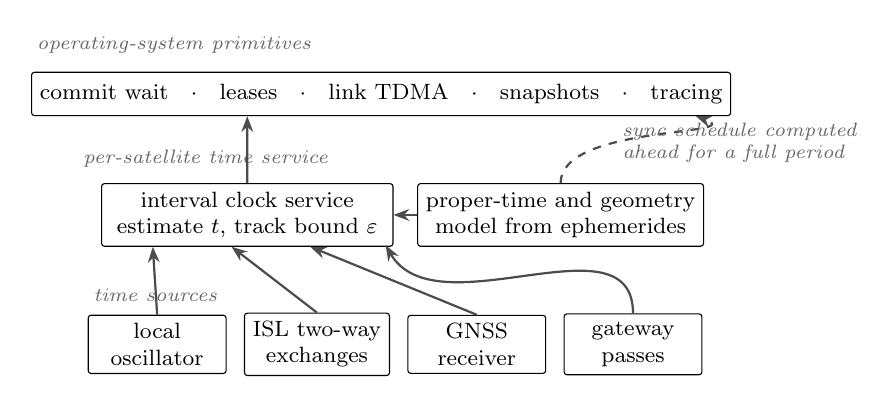
\begin{tikzpicture}[
  font=\footnotesize,
  box/.style={draw, rounded corners=1pt, align=center, inner sep=3pt, minimum height=5.5mm},
  layer/.style={draw=black!60, rounded corners=2pt, inner sep=4pt},
  arr/.style={-{Stealth[length=2mm]}, thick, black!70},
  lbl/.style={font=\scriptsize\itshape, black!60}
]
\def\colw{7.6cm}

% ---- source layer ----
\node[box, minimum width=1.75cm] (osc) {local\\oscillator};
\node[box, minimum width=1.75cm, right=2.2mm of osc] (isl) {ISL two-way\\exchanges};
\node[box, minimum width=1.75cm, right=2.2mm of isl] (gnss) {GNSS\\receiver};
\node[box, minimum width=1.75cm, right=2.2mm of gnss] (gw) {gateway\\passes};
\node[lbl, anchor=west] at ($(osc.west)+(-0.05,0.62)$) {time sources};

% ---- service layer ----
\node[box, minimum width=3.7cm, above=8.5mm of $(isl.north)!0.5!(gnss.north)$, xshift=-1.9cm] (filter)
  {interval clock service\\estimate $t$, track bound $\varepsilon$};
\node[box, minimum width=3.4cm, right=3mm of filter] (model)
  {proper-time and geometry\\model from ephemerides};
\node[lbl, anchor=west] at ($(filter.west)+(-0.35,0.72)$) {per-satellite time service};

% ---- consumer layer ----
\node[box, above=8.5mm of filter.north, xshift=1.7cm, minimum width=7.2cm] (apps)
  {commit wait \; $\cdot$ \; leases \; $\cdot$ \; link TDMA \; $\cdot$ \; snapshots \; $\cdot$ \; tracing};
\node[lbl, anchor=west] at ($(apps.west)+(-0.05,0.62)$) {operating-system primitives};

% ---- arrows ----
\draw[arr] (osc.north) -- ($(filter.south)+(-1.2,0)$);
\draw[arr] (isl.north) -- ($(filter.south)+(-0.2,0)$);
\draw[arr] (gnss.north) -- ($(filter.south)+(0.8,0)$);
\draw[arr] (gw.north) to[out=90,in=-60] ($(filter.south east)+(-0.1,0.02)$);
\draw[arr] (model.west) -- (filter.east);
\draw[arr] (filter.north) -- ($(apps.south)+(-1.7,0)$);

% ---- schedule annotation ----
\draw[arr, dashed] (model.north) to[out=90,in=-20] node[lbl, right, pos=0.35, align=left]
  {sync schedule computed\\ahead for a full period} ($(apps.south east)+(-0.45,0)$);
\end{tikzpicture}
}
\caption{The constellation time stack. Per-satellite interval clocks fuse a local oscillator, scheduled two-way ISL exchanges, GNSS when available, and gateway passes, with corrections and the exchange schedule both derived from ephemerides. Operating-system primitives consume the interval.}
\label{fig:arch}
\end{figure}

\subsection{Time as an Interval}\label{sec:interval}
The service contract is the one TrueTime introduced, a clock read returns an interval guaranteed to contain the true constellation time at the moment of the call~\cite{corbett2012}. Between measurements the half-width $\varepsilon$ grows at the local oscillator's bounded drift rate, and each measurement shrinks it back, giving the familiar sawtooth that Sundial states as $\varepsilon = \varepsilon_{\mathrm{base}} + (t - t_{\mathrm{last}})\cdot y_{\max}$ for drift bound $y_{\max}$~\cite{li2020}. Orbit changes what feeds the equation rather than the equation itself. The drift bound $y_{\max}$ is set by oscillator class and thermal modeling, the refresh events are scheduled link exchanges on a precomputed slot plan, and $\varepsilon$ may vary by orders of magnitude across operating conditions as long as the interval always contains true time. Figure~\ref{fig:holdover} shows the growth arithmetic across oscillator classes and makes the cadence requirement concrete. A calibrated oven-controlled crystal needs a refresh every minute or two to hold 100 ns, which a grid of permanently connected ISLs provides trivially, while a fully isolated satellite with a chip-scale atomic clock crosses a millisecond only after about four weeks, datasheet aging included.

Fusion across sources uses interval intersection, which is four decades old and fits the fault model. Marzullo and Owicki observed that clocks reporting intervals that fail to intersect expose a fault by geometry alone, and that the true time must lie in the intersection of correct intervals~\cite{marzullo1983}. NTP operationalized the idea into an algorithm that finds a majority clique of intersecting intervals among $m$ sources with $f$ falsetickers~\cite{rfc5905}, and Spanner runs a variant in production~\cite{corbett2012}. A satellite fuses its neighbors' exchanges, its GNSS fix when one exists, and gateway time when in view, and a radiation-corrupted clock that jumps simply stops intersecting and is excluded. The tolerance arithmetic is explicit. A node fusing four grid neighbors, a GNSS fix, and an occasional gateway sees five to six sources, and intersection tolerates falsetickers while they stay a minority~\cite{rfc5905}. A satellite that reboots returns with infinite $\varepsilon$ and re-enters receive-only, because scheduled beacons carry slot identity and coarse time, so a blank node listens its way back to microseconds before its first transmission, and a whole-constellation cold start bootstraps the same way from whichever anchors are up. The unscheduled reboots of Section~\ref{sec:break-clock} become routine interval events.

\begin{figure}[t]
\centering
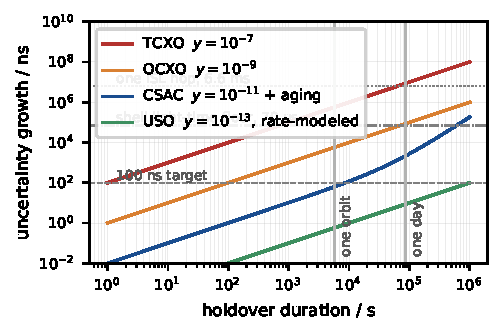
\includegraphics[width=\columnwidth]{figs/fig_holdover.pdf}
\caption{Uncertainty growth during holdover for four oscillator classes, with the chip-scale atomic clock carrying its datasheet aging term, and reference lines at a 100 ns target, at the 6.6 ms light time of one grid hop, at one orbit, and at one day. Oscillator class sets the refresh cadence the fabric must sustain for a given bound, and sets what remains when a satellite is cut off.}
\label{fig:holdover}
\end{figure}

\subsection{Scheduled Exchanges with Geometry as an Input}\label{sec:exchange}
The fabric protocol is a slotted two-way exchange on every grid link, the dual one-way mechanism that satellite time transfer standardized decades ago~\cite{itu1153}, that BeiDou flies between satellites today~\cite{li2025}, and that amounts in IEEE 1588 terms to a hardware-timestamped profile with a deterministic delay model~\cite{ieee1588,whiterabbit}. Our addition is the regime, commodity oscillators, commodity navigation, and an operating system as the consumer. Satellite $A$ records transmit time $a_1$ on its clock, $B$ records arrival $b_1$, replies after a scheduled turnaround $\tau$ at $b_2$, and $A$ records arrival $a_2$. The midpoint estimator
\begin{equation}
\hat\theta \;=\; \tfrac{1}{2}\bigl[(b_1-a_1)-(a_2-b_2)\bigr]
\;=\; \theta \;+\; \tfrac{1}{2}\,(d_1-d_2)
\label{eq:twtt}
\end{equation}
recovers the clock offset $\theta$ exactly when the one-way delays $d_1$ and $d_2$ are equal, which is the assumption NTP makes and cannot defend on terrestrial paths~\cite{mills1991}. In orbit the delays differ because the satellites move during the exchange. The range changes at rate $\dot\rho$, so the return path is longer or shorter than the outgoing one and the estimate acquires a bias
\begin{equation}
\Delta \;=\; \frac{\dot\rho\,(d+\tau)}{2c},
\label{eq:bias}
\end{equation}
with $d=\rho/c$ the one-way flight time. We quote magnitudes throughout, the sign following the geometry. Equation~\ref{eq:bias} reproduces the envelope values of Section~\ref{sec:break-geometry}, 5.4 ns for the padded grid case and 234 ns for a crossing link at 12 km/s. Motion therefore dominates the error budget of orbital time transfer, and it follows deterministically from the relative orbit.

Ephemeris knowledge removes the dominant term. Replacing $\dot\rho$ in Equation~\ref{eq:bias} by the velocity error $\delta\dot\rho$ of the orbit solution gives the residual after correction. The required inputs exist in the fleet today. Starlink satellites estimate their own position autonomously with onboard GPS~\cite{fccgen2}, the operator publishes per-satellite ephemerides through a public repository~\cite{celestrak}, and onboard real-time navigation filters demonstrated on flight data deliver velocity at a few tenths of a millimeter per second~\cite{pod}, with decimeter-class real-time position available from broadcast ephemerides alone~\cite{hauschild2021}. Even at a deliberately conservative $\delta\dot\rho = 1$ cm/s the residual is 0.25 ps on a 3{,}000 km link with a 5 ms turnaround, three orders of magnitude below a nanosecond. Even a full meter per second, worse than any navigation source in the fleet, leaves 25 ps, and the correction only begins to fail beyond tens of meters per second. The remaining relativistic terms are equally well behaved, with the inter-satellite forms derived by Xie~\cite{xie2016}, and Table~\ref{tab:budget} collects the budget. The Shapiro delay on a 3{,}000 km path is 13 ps and cancels in the two-way difference. Satellites in one circular shell share a proper-time rate to first order, eccentricity below $10^{-3}$ contributes a modeled periodic term under 1.2 ns, and the oblateness term stays below half a nanosecond, modeled like the rest. What stops the budget from being arbitrarily small is the hardware. Timestamping at the physical layer with sub-nanosecond calibration is demonstrated engineering, in fiber by White Rabbit~\cite{whiterabbit}, between satellites by the BeiDou-3 crosslinks~\cite{li2025}, and over free space at the femtosecond level by optical two-way transfer~\cite{deschenes2016}. We therefore take 0.1 to 1 ns per link as a conservative fabric residual with physical-layer timestamps, and we treat the absence of such timestamps as a first-class risk in Section~\ref{sec:risks}.

\begin{table}[t]
\centering
\small
\begin{tabular}{@{}lrr@{}}
\toprule
\textbf{Term} & \textbf{Uncorrected} & \textbf{Corrected} \\
\midrule
motion during exchange, grid link & 5.4 ns & $<$1 ps \\
motion during exchange, crossing link & 234 ns & $<$1 ps \\
Shapiro delay, 3{,}000 km path & 13 ps & cancels \\
shell rate difference over exchange & $<$0.1 ps & modeled \\
eccentricity periodic, $e\le10^{-3}$ & 1.2 ns & modeled \\
oblateness periodic & $<$0.5 ns & modeled \\
hardware timestamping and calibration & \multicolumn{2}{c}{0.1 to 1 ns floor} \\
\bottomrule
\end{tabular}
\caption{Two-way exchange error budget on a grid ISL. Corrections use ephemerides with relative velocity known to 1 cm/s and a 5 ms turnaround. Motion dominates uncorrected and vanishes corrected, leaving hardware as the floor.}
\label{tab:budget}
\end{table}

Pairwise residuals compose along the grid into a fleet-level bound, and staleness composes with them. A spanning structure of depth $h$ accumulates at worst $h$ times the per-link residual plus the drift each node accrues between exchanges, $\varepsilon_{\mathrm{fleet}} \le h\,(r + y\,T)$ for residual $r$, drift bound $y$, and slot period $T$, the same depth-proportional engineering Sundial does in a data center~\cite{li2020}. The representative shell has a grid diameter near 47 hops, so at a 0.5 ns residual, oven-controlled discipline at $10^{-9}$, and one exchange per second per link, the worst-case fleet spread sits near 70 ns, and faster slots or better oscillators pull it toward the 24 ns residual floor. Ensemble filtering across the grid's many redundant paths should improve on the worst case, and we leave quantifying that improvement to the evaluation, since geometry alone cannot promise it.

\subsection{Anchors and the Two Timescales}\label{sec:anchors}
Internal agreement and absolute traceability are different products, and the architecture separates them. The fabric of Section~\ref{sec:exchange} maintains the internal timescale, a weighted clock ensemble in the lineage that timing laboratories run for UTC~\cite{lombardi} and that joint-timekeeping work has adapted to crosslinked constellations~\cite{sensors2020}. UTC enters at anchors, meaning gateway contacts and GNSS fixes, and diffuses inward over the same scheduled exchanges, so the constellation's offset from UTC is bounded by anchor quality plus diffusion depth. Per satellite, ground contact is rare, as Section~\ref{sec:break-control} quantified. Per fleet, it is continuous, because at any instant some satellites sit over gateways and every satellite is within tens of hops of one that does.

GNSS is treated as a valuable input rather than a foundation. When receivers track, they hand every satellite an independent absolute fix at the tens-of-nanoseconds level and the fabric's job reduces to smoothing and cross-checking. When receivers degrade, the interval semantics make the degradation explicit, and Section~\ref{sec:risks} weighs how often orbital receivers should actually be expected to degrade. The fabric holds mutual agreement at nanoseconds indefinitely, absolute uncertainty grows only as fast as the anchor ensemble drifts, and every consumer can see exactly how much trust remains, which is the difference between a system that degrades and a system that lies.

\subsection{Predictability as the Operating Principle}\label{sec:predictability}
Everything runtime-fragile in terrestrial synchronization becomes compile-time in orbit, and the architecture leans into this systematically. The exchange schedule for every link, the anchor contact windows, the eclipse entries and exits, and the link-down windows at high latitude or during maneuvers are all functions of ephemerides, so they are computed for a full period ahead and distributed as configuration. The protocol needs no discovery phase and no master election, and topology changes appear in the schedule before they happen. Sundial precomputes a backup parent per node inside a data center to absorb failures locally~\cite{li2020}, and a constellation can precompute every parent for every minute of the next orbit. A maneuver, announced by the operator, becomes a scheduled interval-inflation event on the affected satellite, roughly thirty times per satellite per year at current tempo and one to three kilometers of altitude change each~\cite{pfandzelter2023,maneuvers2025}, and the post-burn ephemeris restores the budget.

The orbital thermal cycle may turn the riskiest parameter of bounded-uncertainty clocks into a modelable one, a hypothesis this paper undertakes to test. Every bounded-uncertainty system stands on its assumed worst-case drift rate, and the published systems set it conservatively because data-center temperature excursions are unpredictable, 200 parts per million in TrueTime and Sundial against quartz that usually drifts far less~\cite{corbett2012,li2020}. A satellite's thermal forcing is periodic at the orbital period, eclipse in and eclipse out, every 95.5 minutes. A per-satellite regression of oscillator frequency against orbital phase, fit continuously from the fabric's own measurements, should capture the systematic component and leave a much smaller stochastic residual, tightening either the achievable bound or the required cadence. Flight data shows the signature we would fit, with analyses of flown LEO clocks finding once-per-revolution and twice-per-revolution periodic residuals at nanosecond amplitudes attributed to relativistic terms, alongside slower multi-hour residuals suspected to track spacecraft temperature~\cite{wang2022}. Whether the remaining residual is small enough to matter is an empirical question, and we state in Section~\ref{sec:risks} what answer would falsify the idea.

Scheduled partitions make leases natural where terrestrial systems find them dangerous. A lease is safe when the holder and the grantor agree the lease has expired before a successor acts, which costs a wait of the uncertainty bound and otherwise costs messages~\cite{liskov1991}. Terrestrial partitions are accidents with unknown duration, so lease-based designs hedge. Orbital partitions are scheduled, a gateway gap or a high-latitude link-down window has a known start, a known end, and a known set of affected nodes, so ownership hand-offs can be placed at instants when the bound is known to be tight and the topology known to be whole.

\subsection{What Bounded Time Buys}\label{sec:buys}
Lamport's inequality stratifies the requirements, and the strata map onto oscillator classes. Anomalous behavior, meaning event orderings that contradict causality carried outside the message system, is eliminated when the synchronization bound stays below the shortest inter-process message time~\cite{lamport1978}, and since no channel beats light, the floor for a satellite pair is the light time at their closest approach. That floor depends on the pair's geometry, with the link graph playing no part. Grid neighbors sit at 6.6 ms, but satellites on crossing tracks within the representative shell pass within roughly 20 to 50 km of each other depending on phasing, light times of 67 to 166 microseconds, and formation-flying satellites 100 m apart sit at a third of a microsecond~\cite{suncatcher2025}. The shell-wide bar is therefore tens of microseconds, which a chip-scale atomic clock holds for about a week of total isolation under its aging spec, an oven-controlled crystal holds for most of a day, and a tracking GNSS receiver clears by three orders of magnitude continuously. Tighter bounds then purchase performance, never correctness. External consistency via commit wait costs one uncertainty width per transaction~\cite{corbett2012}, so a fabric bound of tens of nanoseconds makes the wait five orders of magnitude smaller than the 6.6 to 67 ms of light time a transaction already spends on even a hemisphere-scale path, and ordering becomes purely communication-bound. Sundial quotes FaRMv2's observation that median transaction latency drops 25 percent when the bound falls from 20 microseconds to 100 nanoseconds~\cite{li2020}, and the constellation fabric targets the same regime over physics friendlier than a switched network, because a dedicated point-to-point laser link has no cross traffic and no queueing.

The link layer itself is a time consumer, which closes the circularity noted in Section~\ref{sec:relays}. Guard bands are the clean win, because slotted medium access, beam-hopping schedules, and handover epochs all carry margins sized by clock disagreement plus geometry uncertainty, and nanosecond agreement shrinks them to the geometry term alone. Acquisition gains less than it might appear to. The interoperability standard commercial terminals build to obliges each terminal to carry a clock synchronized to absolute time for its time-tagged spatial search~\cite{sdaoct}, so coarse shared epochs are presupposed by the link layer, and tighter time mostly trims the residual search window. Volume still makes small trims count, with the fleet reporting about 266{,}000 link acquisitions per day in early 2024~\cite{brashears2024} at tens of seconds each~\cite{wu2024,sdaoct}. One fleet-wide timeline also serves observability. Fleet-wide tracing, consistent snapshots, and forensic reconstruction after an upset all want one timeline across 1{,}584 nodes, and hybrid logical clocks supply causality but cannot align records with events outside the message system, ground truth telemetry among them~\cite{kulkarni2014,lamport1978}. An interval clock that is explicit about its bound does both, and degrades by widening.

\subsection{A Sketch of the IPC Layer}\label{sec:ipc}
The clock service exists for the operating system above it, and a research project about that operating system owes a sketch of the layer the clock enables, drawn far enough to test. The first primitive is the channel. Terrestrial inter-process communication discovers its connections at runtime and learns their latency by suffering it, while a constellation channel consults a compiled table, because the contact plan, the routes, and the per-hop light times for the whole next period follow from ephemerides. A send call can therefore return the expected delivery interval before the message leaves, latency becomes a published function of time rather than a measurement, and deadline scheduling of messages reduces to lookup. The published interval holds under an admission policy, because an oversubscribed slot must refuse or re-quote at send time, and silent queueing would break the contract. No terrestrial fabric offers its processes this contract.

Interval timestamps turn the closest-approach floor of Section~\ref{sec:buys} into a free ordering rule for messages. Tag every message with its sender's interval. When two intervals from distinct satellites fail to overlap, midpoint order equals true-time order. When they do overlap, the senders sit within $2\varepsilon$ of simultaneity, and causal influence between distinct satellites needs at least the pairwise light time, so whenever $2\varepsilon$ stays below that floor the overlapping events are guaranteed concurrent and any deterministic tiebreak is a legal serialization~\cite{lamport1978}. All times here are constellation coordinate time, and the concurrency conclusion survives any choice of frame, because spacelike separation does. Cross-satellite timestamp order is then always causally safe, with no agreement protocol and no extra messages. The condition prices itself by geometry, since the 67 microsecond shell floor asks only for $\varepsilon$ under 33 microseconds, which holdover alone sustains for days, while the 0.33 microsecond formation floor asks for $\varepsilon$ under 165 nanoseconds, which needs the fabric or a tracking receiver. Ordering capability degrades with sync class exactly as Section~\ref{sec:buys} stratified.

Shared state binds to absolute time through leases on shards. Each shard of mutable state carries one writer, a lease with an absolute expiry, and a successor the schedule names in advance, in the spirit of Sundial's precomputed backup parents~\cite{li2020}. Handoffs sit at instants the contact plan shows fully connected, renewals cost one message per lease period, and a reboot of the holder costs availability equal to the residual lease plus $2\varepsilon$, claimed by the successor without a message exchanged. Message-free claiming presupposes a synchronously maintained successor replica, so every write pays one extra scheduled message to keep it current, and the availability arithmetic stands conditional on that replication layer, deferred with the rest of the protocol design. Under that condition, at the upset rates of Section~\ref{sec:break-clock}, a ten-second lease, and the expected half-lease residual, a shard loses between 0.1 and 1 second per day, availability between 99.9988 and 99.9999 percent, against a renewal load of a tenth of a message per second plus the per-write replication.

A worked transaction shows where time has gone in the cost structure. A process on one satellite updates a shard owned ten grid hops away, roughly a 15{,}000 km path, and requires external consistency. Propagation alone sets a 50 ms floor each way, per-hop slot waits sit on top, the owner assigns a commit timestamp and waits out the uncertainty, and the acknowledgment returns the same way, a round trip of 100 ms or more. With the fabric's tens-of-nanoseconds bound the commit wait sits six orders of magnitude under the round trip. With TrueTime's terrestrial 4 ms the wait would consume four percent of it~\cite{corbett2012}. With a denied receiver and a bare temperature-compensated oscillator at the $10^{-7}$ class of Section~\ref{sec:break-clock}, the wait would pass 8 ms within a day of holdover and exceed the flight time within a week, at which point ordering cost stops hiding inside communication cost. Timing is invisible in the transaction exactly while the architecture keeps it so.

Computation scheduling inherits the same compiled structure. Moving 100 GB between neighbors takes eight seconds of a 100 Gbps link, and that window is reservable in the same table that schedules exchanges and beams, so placement and transfer planning become static optimization over a known capacity timeline, generalizing the observation that predictable motion rewards planned handover~\cite{bhattacherjee2020}. The sketch stops here deliberately, and it leans on the schedule's accuracy in one way that deserves naming. A satellite that dies silently while the plan still lists it, or drifts from its predicted state through an unmodeled event, voids the assumptions behind message-free claiming until detection catches up, so failure detection and membership join naming, replication protocols, and a process model on the list this sketch defers. The evaluation agenda below exercises the layer's two load-bearing claims, message-free ordering safety and lease availability, in simulation only, a weaker standard than the bench validation the clock receives.

\section{What Could Go Wrong}\label{sec:risks}
We list the ways this proposal fails, in roughly descending order of threat, and for each we state what evidence would change our position.

\runin{GNSS may simply be enough}
The introduction concedes the core of this objection, and this section prices its strongest form. Every satellite can carry a receiver and track absolute time to tens of nanoseconds continuously~\cite{denby2020,pod}, and Section~\ref{sec:buys} shows correctness needs agreement only at the pairwise light-time floor, which GNSS clears in any geometry, by one order of magnitude even in hundred-meter formation and by three in the dispersed shell. The strongest form goes further than absolute time, since GNSS phase common-view between LEO satellites delivers mutual clock agreement below 0.2 ns in real time even on broadcast ephemerides, with no inter-satellite hardware at all~\cite{wang2024cv}, and single-satellite onboard synchronization to GNSS time reaches the sub-nanosecond level on its own~\cite{kunzi2022}. On a fair accounting, a GNSS-trusting operator loses nothing by skipping the fabric, and on arithmetic the fabric loses that contest outright. What the fabric sells is a different good, mutual time whose availability traces to no external signal. The threat evidence for that good needs calibration in turn. The documented interference surge, a 220 percent rise in airline signal-loss events between 2021 and 2024~\cite{gnssjam}, comes from terrestrial receivers near conflict zones, while an orbital receiver looks upward with Earth's horizon attenuating ground-based jammers, so raw jamming threatens a satellite less than an airliner. The cases that remain are spoofing, which may stay credible where brute jamming fades, upset-induced reboots that strip a receiver's fix exactly when the satellite is least able to ask for help~\cite{pfandzelter2023}, correlated receiver faults across a fleet built from one part, and the strategic refusal to depend on another state's signal, the refusal BeiDou acted on with its own crosslinks~\cite{li2025}. Our abandonment criterion splits accordingly. Operational data showing orbital GNSS degradation rare and short enough for chip-scale holdover to bridge would kill the performance case for the fabric, a test we accept, while the sovereignty case rests on procurement posture that no degradation statistic can move.

\runin{The terminals may not expose timestamps}
Sub-nanosecond exchange residuals require timestamping at the optical physical layer, and commercial laser terminals are closed products that may not offer it. White Rabbit needed a modified PHY to reach sub-nanosecond fiber synchronization~\cite{whiterabbit}, and the BeiDou crosslinks that achieve sub-nanosecond comparisons in orbit were purpose-built for it~\cite{li2025}. If deployed terminals expose only application-layer timestamps, queueing and processing jitter put the per-exchange floor at microseconds, the fabric loses two to three orders of magnitude, and GNSS-plus-holdover outperforms it for tightness, leaving the fabric only the independence argument. This is the proposal's binding hardware assumption, and we state it as a requirement on terminal procurement, because the navigation precedent shows the capability flies. The standards are in fact closer than the fear suggests, because the same interoperability document that bounds acquisition obliges terminals to carry an absolute-time clock and to deliver frame timestamps accurate to within 3 ns of the host clock at one-hertz reporting or faster~\cite{sdaoct}, which puts the distance to our 0.1 to 1 ns budget at a factor of three to thirty, while the microsecond cliff applies only to terminals built without such provisions.

\runin{The drift model may not survive flight}
The eclipse-periodic calibration of Section~\ref{sec:predictability} is a hypothesis about oscillator physics in a specific environment, and it can be wrong in several ways. Radiation-induced frequency steps, aging that swamps the periodic term, and attitude-dependent heating that breaks the phase regularity would each leave the regression with little to remove. Terrestrial systems set drift bounds at 200 parts per million for reasons of the same kind~\cite{corbett2012,li2020}. The connected grid rides out this failure, because cadence substitutes for holdover, but the claims about isolated satellites weaken in proportion. A thermal-vacuum testbed running an eclipse profile, or better, telemetry from any operator willing to share oscillator data, settles this cheaply either way.

\runin{Coordination might be designed away instead}
Orbital edge computing in its original form eliminates inter-satellite coordination entirely, assigning each satellite an independent slice of work determined before launch~\cite{denby2020}. If orbital workloads stay embarrassingly parallel, a synchronization fabric has no customer. We find this future possible but narrowing, because the announced systems are link-meshed by design, with Suncatcher requiring aggregate bandwidth near ten terabits per second per link for its training workloads~\cite{suncatcher2025} and deployed constellations routing user traffic over laser grids today~\cite{brashears2024}. Once the links exist, the link layer itself consumes time, and the question stops being whether to synchronize and becomes how well.

\runin{Ephemeris dependence}
The corrections of Section~\ref{sec:exchange} assume orbit knowledge, and the deeper form of this risk is circular, since the velocity sources we cited are themselves GNSS products, which a GNSS-denied fleet loses too. Three exits close the loop. The margin is enormous, since a hundredfold degradation to a full meter per second still leaves the motion residual at 25 ps, and third-party fits to public ephemerides sit near 300 m of position error with no operator data at all~\cite{dyreby2025}. Ground radar tracking feeds orbit determination with no GNSS in its measurement chain. And the fabric measures its own geometry, because the half-sum of the same two-way exchange that compares clocks is a range measurement, which is how BeiDou runs autonomous orbit determination and time synchronization over one crosslink system~\cite{li2025}. Maneuvers remain the stress case, and they arrive announced, roughly thirty per satellite per year at current tempo~\cite{maneuvers2025}, so the schedule inflates the affected intervals and the post-burn ephemeris closes them. Dependence on operator data shapes the architecture, while the numbers themselves carry wide margin.

\runin{The fabric's own trust model}
A fabric motivated by distrust must answer for itself. The exchanges as described carry no authentication, so the design assumes link-layer cryptography on the optical channels, and injecting into a narrow-beam point-to-point laser path is a far harder problem than radiating into an upward-facing GNSS antenna, an asymmetry the architecture leans on and should state. Interval fusion bounds the damage of a subverted or faulty source, because a node fusing five to six sources tolerates a minority of falsetickers~\cite{marzullo1983,rfc5905}, thin headroom that argues for anchor diversity over comfort. The IPC layer of Section~\ref{sec:ipc} inherits the same requirement, because a forged lease claim or a spoofed message timestamp attacks state ownership directly, so lease transfers and timestamps need authentication along with the exchanges. The simulation below therefore injects an adversarial clock alongside the benign fault model.

\runin{A falsifiable agenda}
Three experiments would confirm or kill the proposal, and we commit to the kill criteria in advance. First, simulation. Extending Hypatia~\cite{kassing2020} with oscillator noise, exchange schedules, and fault injection at published upset rates~\cite{pfandzelter2023} tests whether a 72 by 22 shell holds a 100 ns mutual bound for 99 percent of satellite pairs through high-latitude link churn, maneuvers, reboots, and one adversarially wrong clock, and measures end-to-end transaction latency and shard availability from Section~\ref{sec:ipc} alongside the bound. The proposal fails here if depth-47 accumulation defeats ensemble averaging. Second, a two-node hardware exchange over an emulated moving channel, validating Equation~\ref{eq:bias} and its correction against injected ephemeris error, with the stated limitation that a bench reproduces neither vacuum nor the thermal swing of eclipse. The proposal fails here if terminal-internal delays prove uncalibratable below several nanoseconds. Third, the thermal regression on flight or chamber data as above, with a factor-of-two reduction in holdover error as the bar for mattering. Each experiment is independently publishable, none requires launching anything, and the first two are within reach of a university lab.

\section{Related Work}\label{sec:related}
Navigation constellations have crossed the line this paper argues orbital data centers must cross, which is satellites keeping time among themselves. GPS Block IIR carried AutoNav, crosslink ranging and onboard estimation designed to hold accuracy through 180 days without ground contact~\cite{autonav}. BeiDou-3 satellites compare clocks over Ka-band crosslinks in three-second dual one-way slots, with validation on a GEO crosslink near 0.1 ns and crosslink hardware biases stable at 0.2 ns, while reducing dependence on a regionally constrained ground network~\cite{li2025}, and joint-timekeeping work builds a constellation timescale from such comparisons as a weighted clock ensemble~\cite{sensors2020}. The motive carries a lesson for compute constellations, since a navigation system supplies the signal everyone else leans on and cannot bootstrap from one, while an orbital data center faces the same independence as a choice rather than a necessity. The Kepler concept for next-generation satellite navigation goes further, proposing optical ISLs and cavity-stabilized lasers with Allan deviation near $10^{-15}$ so that the constellation synchronizes itself at the picosecond level and the ground segment shrinks to a single station~\cite{gunther2018}. These systems prove the physics and the engineering in flight. They differ from our setting in product and in hardware class, since for them time is the payload, justifying premium frequency references on a few dozen satellites, while an orbital data center needs time as infrastructure across thousands of commodity nodes, consumed by software through an explicit uncertainty contract.

The ceilings of time-transfer physics sit far above what this proposal asks for. The ACES mission, launched to the International Space Station in April 2025, operates a microwave space-to-ground link whose carrier-phase comparisons reach 60 femtoseconds of time deviation at ten seconds and stay below a picosecond long term~\cite{aces,cacciapuoti2024}. Optical two-way transfer over a turbulent four-kilometer free-space path holds clocks matched to below a femtosecond~\cite{deschenes2016}, and White Rabbit delivers sub-nanosecond accuracy with ten-picosecond class jitter over kilometers of fiber as an Ethernet service~\cite{whiterabbit}. Against these demonstrations, the 0.1 to 1 ns per-link residual this paper budgets qualifies as a conservative engineering target.

Data-center synchronization supplies the abstraction this paper ports to orbit, under assumptions that invert. TrueTime, Huygens, Sundial, and hybrid logical clocks together map the design space of bounded, measured, or causality-only time on the ground~\cite{corbett2012,geng2018,li2020,kulkarni2014}, and all of them fight a network whose topology is fixed but whose delays are stochastic. The constellation presents the mirror image, a topology in constant motion with delays that are deterministic functions of time, computable from ephemerides to better than a nanosecond. The interval semantics carry over unchanged. The measurement machinery underneath them changes completely, from statistical filtering against queueing noise to geometric correction against known motion, which makes the fabric an IEEE 1588 hardware-timestamping profile whose delay model comes from orbital mechanics~\cite{ieee1588,whiterabbit}.

LEO networking research recognizes orbital predictability as a lever, and the missing piece sits between fields. Navigation practice already applies predicted orbits to time comparison operationally~\cite{li2025,itu1153}, and the synchronization survey literature catalogs techniques for distributed satellite systems~\cite{survey2022}. On the computing side, Hypatia builds its simulation around deterministic orbital motion~\cite{kassing2020}, topology design exploits stable relative geometry for grid ISLs~\cite{bhattacherjee2019}, the failure-model literature catalogs what breaks in orbit~\cite{pfandzelter2023}, and the ISL survey literature states plainly that predictable trajectories should drive pre-scheduled handover and routing~\cite{wu2024}, noting that crosslink ranging enhances time synchronization of the space segment and stopping there. Two adjacent positions complete the map, a proposal for satellites as a clock product serving the ground~\cite{ducoing2023}, the mirror image of time as internal infrastructure, and Mills's early sketch of NTP-style time service over space data links with orbital-mechanics prediction~\cite{millspits}. We read this body of work as having built every piece of the argument except the conclusion, that a compute constellation should keep time through the links it flies, on a schedule its geometry fixes, behind an interval contract its software can consume.

\section{Conclusion \& Future Work}\label{sec:conclusion}
A constellation that computes needs an answer to the oldest question in distributed systems, and the answer it inherits from GPS does not transfer. We made the GPS timekeeping architecture's assumptions explicit, premium clocks, a watching ground, one-way time flow, factory-constant relativity, and an external consumer, and showed quantitatively that an orbital data center violates all five. The same orbital mechanics that breaks ground-centric correction supplies the fix, because it makes the constellation an unusually prediction-friendly environment for a synchronization protocol, the dominant error of two-way transfer between satellites being their known motion. Our error budget shows ephemeris-corrected exchanges over existing grid ISLs leaving sub-picosecond motion residuals against a hardware floor near a nanosecond, satellites in one shell sharing a single relativistic rate, and agreement at the inter-satellite light time sufficing for correctness while the nanosecond regime purchases commit-wait costs five orders of magnitude under light time, tighter link schedules, and one fleet-wide timeline for observability.

Constellation time, the architecture we propose, packages these facts behind the interval abstraction that terrestrial systems have proven, with uncertainty explicit, fusion by intersection, anchors absorbed rather than trusted, and every schedule computed ahead from geometry. Above it sits the layer the project is actually about, channels whose latency is published in advance, message ordering made causally safe by the same light-time floors, and leases that hand state across reboots without a message. The fabric is for the operator who refuses that external dependence, and the interval and modeling layers apply under any operator. The proposal can be wrong in named ways, and Section~\ref{sec:risks} attaches an experiment or stated evidence to each. Two of the three experiments need only a lab, and the third needs only oscillator telemetry an operator already records. That is where we will start.

\small
\begin{thebibliography}{99}
\itemsep 1pt plus 0.3pt

\bibitem{mcdowellstats}
Jonathan McDowell.
Starlink launch statistics.
Jonathan's Space Pages, data updated June 10, 2026.
\url{https://planet4589.org/space/con/star/stats.html}

\bibitem{brashears2024}
Michael Kan.
Starlink's laser system is beaming 42 million GB of data per day.
\textit{PC Magazine}, January 30, 2024. Reporting Travis Brashears, SpaceX, at SPIE Photonics West 2024.
\url{https://www.pcmag.com/news/starlinks-laser-system-is-beaming-42-million-gb-of-data-per-day}

\bibitem{denby2020}
Bradley Denby and Brandon Lucia.
Orbital edge computing: Nanosatellite constellations as a new class of computer system.
In \textit{Proc.\ ASPLOS}, 2020.
\url{https://brandonlucia.com/pubs/oec-asplos2020.pdf}

\bibitem{bhattacherjee2020}
Debopam Bhattacherjee, Simon Kassing, Melissa Licciardello, and Ankit Singla.
In-orbit computing: An outlandish thought experiment?
In \textit{Proc.\ ACM HotNets}, 2020.
\url{https://people.computing.clemson.edu/~jmarty/projects/lowLatencyNetworking/papers/LEO-Sat-Broadband-Access/InOrbitComputingAnOutlandishThoughtExperiment.pdf}

\bibitem{suncatcher2025}
Blaise Ag\"uera y Arcas, Travis Beals, Maria Biggs, Jessica V. Bloom, Thomas Fischbacher, Konstantin Gromov, Urs K\"oster, Rishiraj Pravahan, and James Manyika.
Towards a future space-based, highly scalable AI infrastructure system design.
arXiv:2511.19468, November 2025.
\url{https://arxiv.org/abs/2511.19468}

\bibitem{starcloud2025}
Tereza Pultarova.
NVIDIA's H100 GPU takes data centers to space.
\textit{IEEE Spectrum}, November 3, 2025.
\url{https://spectrum.ieee.org/nvidia-h100-space}

\bibitem{spacenews2026}
Jeff Foust.
SpaceX files plans for million-satellite orbital data center constellation.
\textit{SpaceNews}, January 31, 2026.
\url{https://spacenews.com/spacex-files-plans-for-million-satellite-orbital-data-center-constellation/}

\bibitem{lamport1978}
Leslie Lamport.
Time, clocks, and the ordering of events in a distributed system.
\textit{Communications of the ACM}, 21(7):558--565, 1978.
\url{https://lamport.azurewebsites.net/pubs/time-clocks.pdf}

\bibitem{liskov1991}
Barbara Liskov.
Practical uses of synchronized clocks in distributed systems.
\textit{Distributed Computing}, 6(4):211--219, 1993. Originally in \textit{Proc.\ ACM PODC}, 1991.
\url{https://link.springer.com/article/10.1007/BF02242709}

\bibitem{kassing2020}
Simon Kassing, Debopam Bhattacherjee, Andr\'e Baptista \'Aguas, Jens Eirik Saethre, and Ankit Singla.
Exploring the ``Internet from space'' with Hypatia.
In \textit{Proc.\ ACM IMC}, 2020.
\url{https://bdebopam.github.io/papers/imc2020-hypatia.pdf}

\bibitem{pfandzelter2023}
Tobias Pfandzelter and David Bermbach.
Edge computing in low-Earth orbit -- what could possibly go wrong?
In \textit{Proc.\ ACM LEO-NET}, 2023. arXiv:2302.08952.
\url{https://arxiv.org/abs/2302.08952}

\bibitem{ashby2003}
Neil Ashby.
Relativity in the Global Positioning System.
\textit{Living Reviews in Relativity}, 6(1), 2003.
\url{https://link.springer.com/article/10.12942/lrr-2003-1}

\bibitem{gpscontrol}
National Coordination Office for Space-Based Positioning, Navigation, and Timing.
GPS control segment.
Accessed June 2026.
\url{https://www.gps.gov/control-segment}

\bibitem{pod}
Fuhong Wang, Xuewen Gong, Jizhang Sang, and Xiaohong Zhang.
A novel method for precise onboard real-time orbit determination with a standalone GPS receiver.
\textit{Sensors}, 15(12):30403--30418, 2015.
\url{https://europepmc.org/article/MED/26690149}

\bibitem{fccgen2}
Space Exploration Holdings, LLC.
Application for approval of the SpaceX Gen2 NGSO satellite system, technical attachment.
FCC IBFS SAT-LOA-20200526-00055, May 2020.
\url{https://fcc.report/IBFS/SAT-LOA-20200526-00055/2378671.pdf}

\bibitem{li2025}
Jie Li, Jun Zhu, Rengui Ruan, Xiaolong Xu, Yanan Fang, Chong Wang, and Zongbo Huyan.
Application and accuracy analysis of raw one way inter-satellite link observations of BDS-3 full operational constellation.
\textit{Scientific Reports}, 15:14438, 2025.
\url{https://www.nature.com/articles/s41598-025-98560-5}

\bibitem{itu1153}
International Telecommunication Union.
The operational use of two-way satellite time and frequency transfer employing PN codes.
Recommendation ITU-R TF.1153-4, August 2015.
\url{https://www.itu.int/rec/R-REC-TF.1153/en}

\bibitem{corbett2012}
James C. Corbett, Jeffrey Dean, Michael Epstein, et al.
Spanner: Google's globally-distributed database.
In \textit{Proc.\ USENIX OSDI}, 2012.
\url{https://static.googleusercontent.com/media/research.google.com/en//archive/spanner-osdi2012.pdf}

\bibitem{turyshev2026}
Slava G. Turyshev.
Orbital data centers: Spacecraft constraints and economic viability.
arXiv:2604.27197, April 2026.
\url{https://arxiv.org/abs/2604.27197}

\bibitem{bhattacherjee2019}
Debopam Bhattacherjee and Ankit Singla.
Network topology design at 27,000 km/hour.
In \textit{Proc.\ ACM CoNEXT}, 2019.
\url{https://bdebopam.github.io/papers/conext19_LEO_topology.pdf}

\bibitem{geng2018}
Yilong Geng, Shiyu Liu, Zi Yin, Ashish Naik, Balaji Prabhakar, Mendel Rosenblum, and Amin Vahdat.
Exploiting a natural network effect for scalable, fine-grained clock synchronization.
In \textit{Proc.\ USENIX NSDI}, 2018.
\url{https://www.usenix.org/system/files/conference/nsdi18/nsdi18-geng.pdf}

\bibitem{li2020}
Yuliang Li, Gautam Kumar, Hema Hariharan, et al.
Sundial: Fault-tolerant clock synchronization for datacenters.
In \textit{Proc.\ USENIX OSDI}, 2020.
\url{https://www.usenix.org/system/files/osdi20-li_yuliang.pdf}

\bibitem{kulkarni2014}
Sandeep Kulkarni, Murat Demirbas, Deepak Madeppa, Bharadwaj Avva, and Marcelo Leone.
Logical physical clocks and consistent snapshots in globally distributed databases.
Technical Report 2014-04, University at Buffalo CSE, 2014. Also in \textit{Proc.\ OPODIS}, 2014.
\url{https://cse.buffalo.edu/tech-reports/2014-04.pdf}

\bibitem{gpssps}
U.S. Department of Defense.
Global Positioning System standard positioning service performance standard, 5th edition.
April 2020.
\url{https://www.gps.gov/sites/default/files/2025-07/2020-SPS-performance-standard.pdf}

\bibitem{pascual2005}
J.-F. Pascual-S\'anchez.
Introducing relativity in global navigation satellite systems.
\textit{Annalen der Physik}, 16(4):258--273, 2007. arXiv:gr-qc/0507121.
\url{https://arxiv.org/abs/gr-qc/0507121}

\bibitem{kuiper}
Rachel Jewett.
Second ULA launch brings Amazon Kuiper constellation to 54 satellites.
\textit{Via Satellite}, June 23, 2025.
\url{https://www.satellitetoday.com/launch/2025/06/23/second-ula-launch-brings-amazon-kuiper-constellation-to-54-satellites/}

\bibitem{wu2024}
Chenyu Wu, Shuai Han, Qian Chen, Yu Wang, Weixiao Meng, and Abderrahim Benslimane.
Enhancing LEO mega-constellations with inter-satellite links: Vision and challenges.
arXiv:2406.05078, June 2024.
\url{https://arxiv.org/abs/2406.05078}

\bibitem{wang2022}
Kan Wang and Ahmed El-Mowafy.
LEO satellite clock analysis and prediction for positioning applications.
\textit{Geo-spatial Information Science}, 25(1):14--33, 2022.
\url{https://www.tandfonline.com/doi/full/10.1080/10095020.2021.1917310}

\bibitem{csac}
Microchip Technology Inc.
SA.45s chip-scale atomic clock datasheet, parts 090-03240-001 and 090-03240-003.
2019.
\url{https://media.digikey.com/pdf/Data\%20Sheets/Microchip\%20PDFs/090-03240-001,\%20090-03240-003.pdf}

\bibitem{mills1991}
David L. Mills.
Internet time synchronization: The network time protocol.
\textit{IEEE Transactions on Communications}, 39(10):1482--1493, 1991.
\url{https://www.ntp.org/reflib/papers/trans.pdf}

\bibitem{maneuvers2025}
Advanced Television.
Starlink explains real risks of orbital collision.
July 30, 2025. Reporting SpaceX's semi-annual constellation status report to the FCC.
\url{https://www.advanced-television.com/2025/07/30/starlink-explains-real-risks-of-orbital-collision/}

\bibitem{marzullo1983}
Keith Marzullo and Susan Owicki.
Maintaining the time in a distributed system.
In \textit{Proc.\ ACM PODC}, 1983.
\url{https://www.uio.no/studier/emner/matnat/ifi/IN5570/v22/teaching-materials/p44-marzullo.pdf}

\bibitem{rfc5905}
David L. Mills, Jim Martin, Jack Burbank, and William Kasch.
Network time protocol version 4: Protocol and algorithms specification.
RFC 5905, IETF, June 2010.
\url{https://www.rfc-editor.org/rfc/rfc5905.txt}

\bibitem{ieee1588}
IEEE.
IEEE standard for a precision clock synchronization protocol for networked measurement and control systems.
IEEE Std 1588-2019.
\url{https://standards.ieee.org/ieee/1588/6825/}

\bibitem{whiterabbit}
Maciej Lipi\'nski, Tomasz W\l{}ostowski, Javier Serrano, and Pablo Alvarez.
White Rabbit: A PTP application for robust sub-nanosecond synchronization.
In \textit{Proc.\ IEEE ISPCS}, 2011.
\url{https://white-rabbit.web.cern.ch/documents/White_Rabbit-a_PTP_application_for_robust_sub-nanosecond_synchronization.pdf}

\bibitem{celestrak}
T.~S. Kelso.
Supplemental GP element sets.
CelesTrak. Accessed June 2026.
\url{https://celestrak.org/NORAD/elements/supplemental/}

\bibitem{hauschild2021}
Andr\'e Hauschild and Oliver Montenbruck.
Precise real-time navigation of LEO satellites using GNSS broadcast ephemerides.
\textit{NAVIGATION}, 68(2):419--432, 2021.
\url{https://navi.ion.org/content/navi/68/2/419.full.pdf}

\bibitem{xie2016}
Yi Xie.
Relativistic time transfer for inter-satellite links.
\textit{Frontiers in Astronomy and Space Sciences}, 3:15, 2016.
\url{https://www.frontiersin.org/journals/astronomy-and-space-sciences/articles/10.3389/fspas.2016.00015/full}

\bibitem{deschenes2016}
Jean-Daniel Desch\^enes, Laura C. Sinclair, Fabrizio R. Giorgetta, William C. Swann, Esther Baumann, Hugo Bergeron, Michael Cermak, Ian Coddington, and Nathan R. Newbury.
Synchronization of distant optical clocks at the femtosecond level.
\textit{Physical Review X}, 6:041016, 2016. arXiv:1509.07888.
\url{https://arxiv.org/abs/1509.07888}

\bibitem{lombardi}
Michael A. Lombardi.
Fundamentals of time and frequency.
In \textit{The Mechatronics Handbook}, CRC Press, 2002. Hosted by NIST.
\url{https://tf.nist.gov/general/pdf/1498.pdf}

\bibitem{sensors2020}
Leyuan Sun, Wende Huang, Shuaihe Gao, Wei Li, Xiye Guo, and Jun Yang.
Joint timekeeping of navigation satellite constellation with inter-satellite links.
\textit{Sensors}, 20(3):670, 2020.
\url{https://europepmc.org/article/MED/31991743}

\bibitem{sdaoct}
Space Development Agency.
Optical communications terminal (OCT) standard, version 4.0.0.
July 2024.
\url{https://www.sda.mil/wp-content/uploads/2024/07/SDA_OCT_Standard_4.0.0_final-20240701.pdf}

\bibitem{wang2024cv}
Kan Wang, Baoqi Sun, Ahmed El-Mowafy, and Xuhai Yang.
High-precision time transfer and relative orbital determination among LEO satellites in real time.
\textit{NAVIGATION}, 71(3), 2024.
\url{https://navi.ion.org/content/71/3/navi.659}

\bibitem{kunzi2022}
Florian Kunzi and Oliver Montenbruck.
Precise onboard time synchronization for LEO satellites.
\textit{NAVIGATION}, 69(3), 2022.
\url{https://navi.ion.org/content/69/3/navi.531}

\bibitem{gnssjam}
European Union Aviation Safety Agency and International Air Transport Association.
EASA and IATA outline comprehensive plan to mitigate GNSS interference risks.
Press release, June 18, 2025.
\url{https://www.easa.europa.eu/en/newsroom-and-events/press-releases/easa-and-iata-outline-comprehensive-plan-mitigate-gnss}

\bibitem{dyreby2025}
Katarina Dyreby, Francisco Caldas, and Cl\'audia Soares.
Analyzing data quality and decay in mega-constellations: A physics-informed machine learning approach.
arXiv:2510.11242, October 2025.
\url{https://arxiv.org/abs/2510.11242}

\bibitem{autonav}
GlobalSecurity.org.
GPS Block IIR AutoNav.
National Security Space Road Map initiative description, 1999.
\url{https://www.globalsecurity.org/space/library/report/1999/nssrm/initiatives/gps2r.htm}

\bibitem{gunther2018}
Christoph G\"unther.
Kepler -- satellite navigation without clocks and ground infrastructure.
In \textit{Proc.\ ION GNSS+}, 2018.
\url{https://elib.dlr.de/126622/1/Kepler_ION18_C.pdf}

\bibitem{aces}
European Space Agency.
ACES: Atomic Clock Ensemble in Space.
Accessed June 2026.
\url{https://www.esa.int/Science_Exploration/Human_and_Robotic_Exploration/ACES_Atomic_Clock_Ensemble_in_Space}

\bibitem{cacciapuoti2024}
Luigi Cacciapuoti et al.
Atomic Clock Ensemble in Space.
arXiv:2411.02912, November 2024.
\url{https://arxiv.org/abs/2411.02912}

\bibitem{survey2022}
Liz Martinez Marrero, Juan C. Merlano Duncan, Jorge Querol, Sumit Kumar, Jevgenij Krivochiza, Shree Krishna Sharma, et al.
Architectures and synchronization techniques for distributed satellite systems: A survey.
\textit{IEEE Access}, 2022. arXiv:2203.08698.
\url{https://arxiv.org/abs/2203.08698}

\bibitem{ducoing2023}
Sage Ducoing, Ivan Agullo, James E. Troupe, and Stav Haldar.
A quantum-assisted master clock in the sky: Global synchronization from satellites at sub-nanosecond precision.
arXiv:2311.11155, 2023.
\url{https://arxiv.org/abs/2311.11155}

\bibitem{millspits}
David L. Mills.
Time synchronization for space data links.
University of Delaware project page.
\url{https://www.eecis.udel.edu/~mills/proximity.html}

\end{thebibliography}

\end{document}
